\documentclass{standalone}
\usepackage{pgfplots}
\pgfplotsset{compat=newest}

\begin{document}
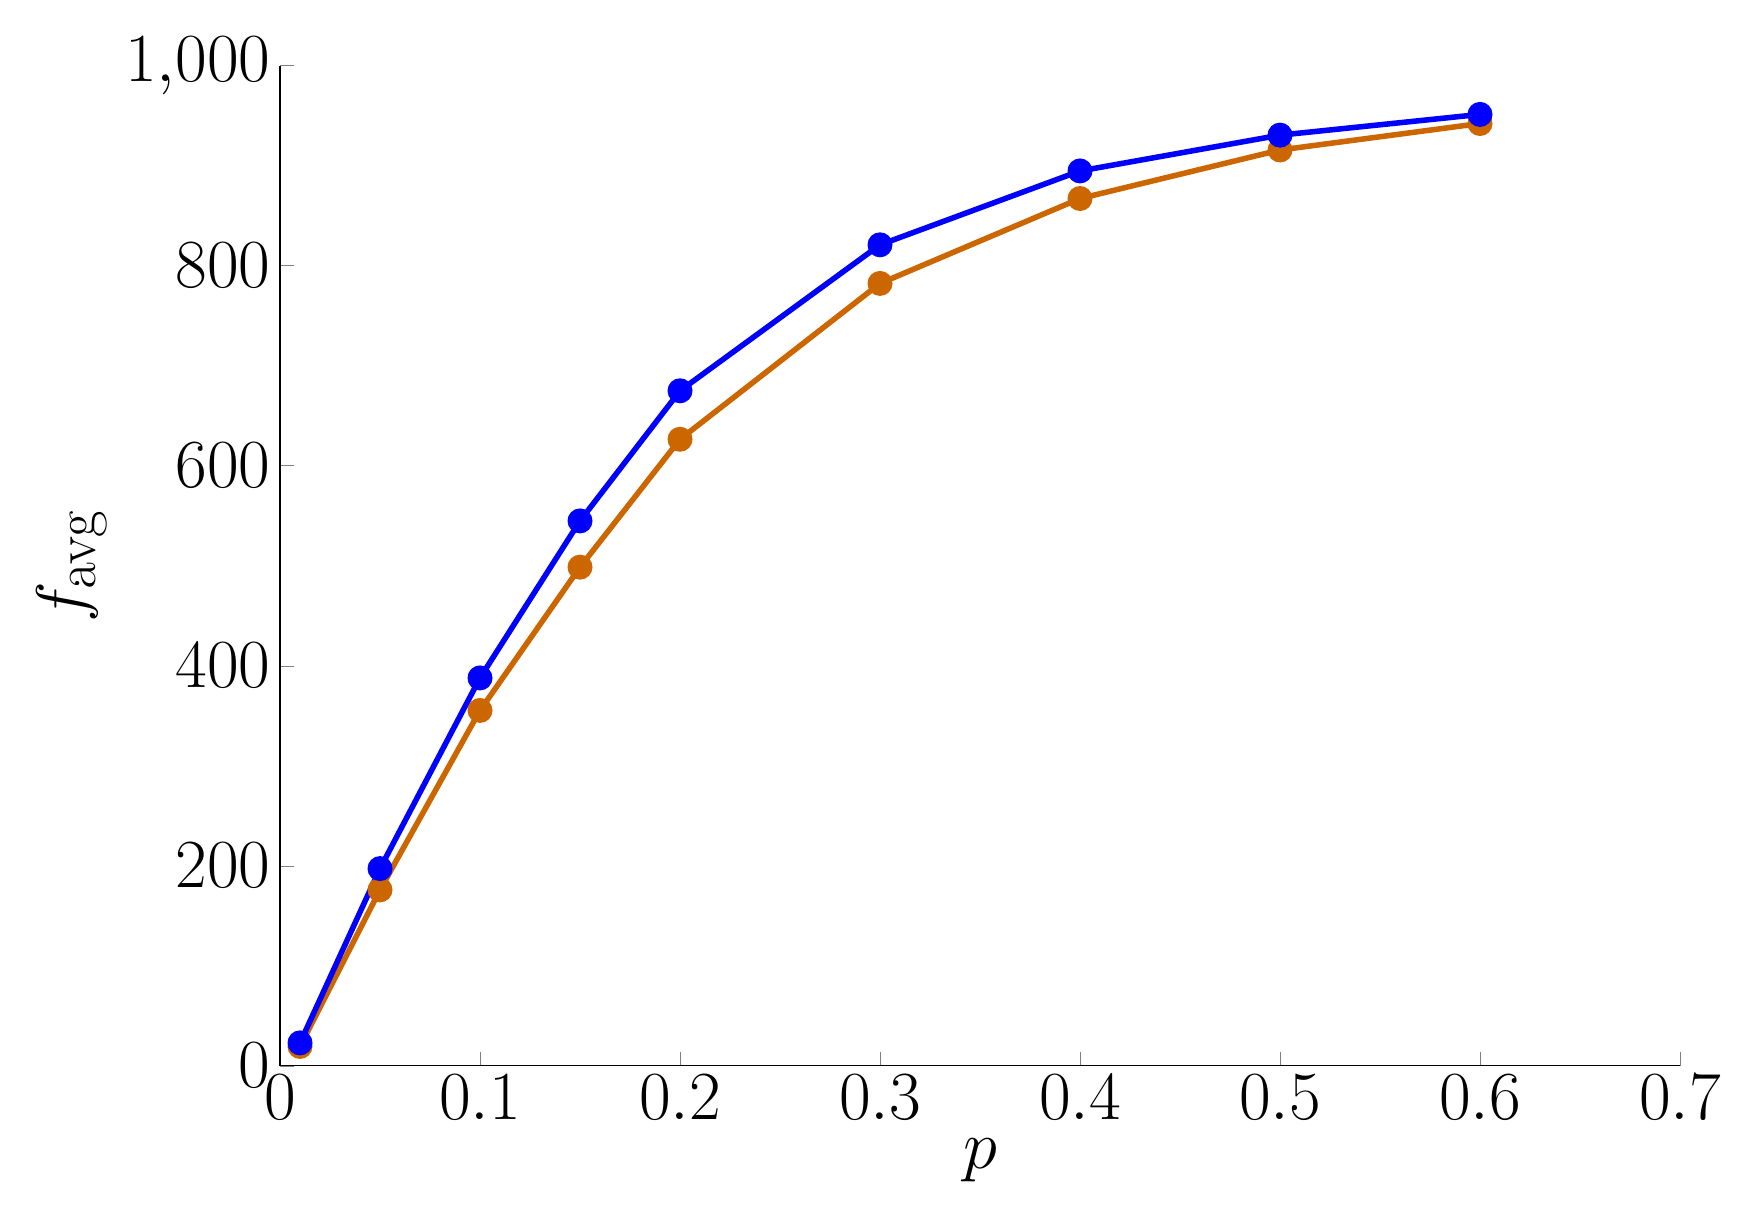
\begin{tikzpicture}

\begin{axis}[%
tick label style={font=\Huge},
label style={font=\Huge},
legend style={font=\Huge},
view={0}{90},
width=7in,
height=5in,
scale only axis,
xmin=0, xmax=0.7,
xtick={0, 0.1, 0.2, 0.3, 0.4, 0.5, 0.6, 0.7},
xlabel={$p$},
ymin=0, ymax=1000,
ytick={0, 200, 400, 600, 800, 1000},
ylabel={$f_{\mathrm{avg}}$},
major tick length=5pt,
axis lines*=left,
legend cell align=left,
clip=false]

%% \addplot [
%% draw=none,
%% fill=orange!80!black,
%% opacity=0.5,
%% solid,
%% line width=2pt
%% ]
%% coordinates{
%% %std_nonad%
%% };

%% \addplot [
%% draw=none,
%% fill=blue,
%% opacity=0.5,
%% solid,
%% line width=2pt
%% ]
%% coordinates{
%% %std_ad%
%% };

\addplot [
mark=*,
mark size=3.5pt,
color=orange!80!black,
solid,
line width=2pt,
]
coordinates{
(0.01,19.31)(0.05,175.9)(0.1,355.35)(0.15,498.63)(0.2,626.5)(0.3,782.34)(0.4,867.23)(0.5,915.78)(0.6,942.25)
};

\addplot [
mark=*,
mark size=3.5pt,
color=blue,
solid,
line width=2pt,
]
coordinates{
(0.01,22.89)(0.05,197.2)(0.1,387.85)(0.15,544.87)(0.2,674.98)(0.3,820.96)(0.4,894.83)(0.5,930.63)(0.6,951.37)
};

\end{axis}
\end{tikzpicture}
\end{document}
